\documentclass[pdftex,12pt,letter]{article}
\usepackage{fancyhdr}
\usepackage{enumerate}
\usepackage{tabularx}
\usepackage{graphicx}
\usepackage{array}
\usepackage[justification=justified,singlelinecheck=false]{caption}
\usepackage{placeins}
\pagestyle{fancy}
\makeatletter
  \renewcommand\@seccntformat[1]{\csname the#1\endcsname.\quad}
\makeatother

\newcolumntype {Y}{ >{\raggedright \arraybackslash }X}
\newcommand{\HRule}{\rule{\linewidth}{0.5mm}}
\captionsetup{labelformat=empty}

\begin{document}

\begin{titlepage}
\begin{flushright}
\HRule \\[0.4cm]
{ \bfseries
{\huge Functional Test Requirements\\[1cm]}
{\Large for\\[1cm]}
{\huge CWRUtility\large\\[4cm]}
{\large Prepared by\\Jason Kuster, Stuart Long, and William Ordiway\\[1cm]
Version 1.0\\[1cm]
KOALAA Development\\[1cm]
November 12, 2012}}
\end{flushright}
\end{titlepage}
\tableofcontents{}
\begin{table}[!t]
\caption*{\bfseries Revision History}
\begin{tabularx}{\textwidth }[t]{|l|Y|Y|l|}
\hline
\bfseries Name & \bfseries Date & \bfseries Reasons for Change & \bfseries Version \\ \hline
Long & 9/22/2012 & Initial Draft & 1.0a\\
\hline
\end{tabularx}
\end{table}
\FloatBarrier
\newpage
\clearpage
\section{Main Page}
\begin{enumerate}[1.]
\item When opened, the application will display the main page.
\item From the main page, the user will be able to select any of the rest of the features of the application.
\item When the user selects a feature, the application will switch from the main page to that feature.
\item If a user "sets defaults" in either the \emph{eSuds} or \emph{NextBus} feature, the main page will accurately display the appropriate information next to the respective feature. (See the \emph{eSuds} and \emph{NextBus} for more information)
\item From any of the other features, if the user hits the "back" button, the user will be returned to the main page.
\end{enumerate}
\section{NextBus}
\begin{enumerate}[1.]
\item The user will be able to view the next 3 prediction times for the NextBus shuttles on campus.
\item The user will be able to select a bus route from the first list box.
\item The user will be able to select a route direction from the second list box.
\item The user will be able to select a stop from the third list box.
\item Upon pressing "Go", the predictions for the bus at that stop will be displayed.
\item If the bus has ceased to run for the day, this will be indicated.
\item The user will be able to select the "add favorite" button at the bottom of the page, which will set the default location upon navigation to the NextBus page, as well as the bus stop which will be displayed on the main page.
\end{enumerate}
\section{Campus Map}
\begin{enumerate}[1.]
\item The user will be able to either view a "Bing" map of the CWRU campus or an offical CWRU map of the CWRU campus.
\item The user will be able to swipe laterally to switch between the two maps.
\item On the "bing" map, the user will be able to zoom-in by putting two fingers on the phone and moving them away from each other.
\item On the "bing" map, the user will be able to zoom-out by putting two fingers on the phone and moving them towards each other.
\item On the "bing" map, the user will be able to pan the map by placing a single finger on the phone and moving it parallel to the direction the user wishes to pan.
\item The "bing" map will display a campus outline and several campus landmarks using pushpins.
\item The user will be able to hide this outline and these pushpins by tapping the "toggle info" button.
\item Once hidden the user will be able to display the outline and pushpins by tapping the "toggle info" button again.
\item The user will be able to tap the "my location" button, and the application will display the user's current location on the "bing" map.
\item The "toggle info" button will also affect the visibility of the pushpin representing the user's current location.
\item On the official CWRU map, the user will be able to pan around the map at will in the same manner as on the "bing" map.
\item The user will be able to return to the main page by hitting the phone's "back" button.
\end{enumerate}
\section{eSuds}
\begin{enumerate}[1.]
\item The user will be able to view a list box of washer and dryer statuses.
\item The user will be able to select a building from a dropdown menu.
\item Upon selecting a building, the washer and dryer statuses will update for the selected building.
\item In the case that the list of washers and dryers overflows the listbox, the user will be able to swipe their finger vertically to scroll through the list.
\item The user will be able to select the "add favorite" button at the bottom of the page, which will set the default location upon navigation to the eSuds page, as well as the building whose free washer/dryer count will be displayed on the main page.
\end{enumerate}
\section{Directory}
\begin{enumerate}[1.]
\item The user will be presented with a list of names of campus resources.
\item The user will be able to swipe vertically to scroll through the list.
\item Tapping a resource name reveals an address, phone number, and a short description of that resource.
\item If a resource name is tapped and its information is revealed beyond the view on the phone it will auto scroll so this information is on the screen.
\item If an already opened resource is tapped it will collapse.
\item If a new resource is tapped it will collapse the previously opened resource.
\item If a phone number is tapped it will bring up a dialog box presenting the user with the option of calling that phone number.
\item The user will be able to return to the main page by hitting the phone's "back" button.
\item  If the user opens the "Directory" again from the main page after having it open previously they will be presented with a list of names of campus resources with all other information collapsed as if they had just opened the feature for the first time.
\end{enumerate}
\section{Menus}
\begin{enumerate}[1.]
\item The user will be presented with the menu for Leutner for the current date generated from the RSS feed from Bon Appetit. 
\item The user may swipe horizontally to change the view from Leutners menu to Fribley's menu.
\item The user may select a date from a dropbox at the bottom of the page.
\item These dates will be the days of the current week, as generated by the Windows Phone
\item Upon selection of a day the Menus page will reload and display the menu for that day. Bon Appetit provides menus for all of the days of the current week.
\item The user may tap a "refresh feed" button to manually refresh the RSS feed.
\item While feeds are being refreshed, the user will see a progress bar at the top of the application.
\item The user will be able to return to the main page by hitting the phone's "back" button.
\end{enumerate}
\section{Case News}
\begin{enumerate}[1.]
\item The user will be able to view an RSS feed from both \emph{The Observer} and \emph{The Case Daily}. 
\item The user will be able to switch between view stories from either news source by swiping laterally on the phone.
\item The user will be able to tap on a news story and the application will switch to a new page that displays the story in its entirety.
\item On being opened, this feature will automatically refresh the feed of the current RSS feed.
\item The user will be able to tap the "refresh feed" button to manually refresh the RSS feed of the current feed.
\item While feeds are being refreshed, the user will see a progress bar at the top of the application.
\item The user will be able to return to the main page by hitting the phone's "back" button.
\end{enumerate}
\lfoot{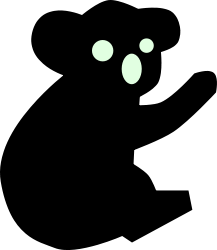
\includegraphics[height=1cm]{DarkKoala.png}}
\end{document}